\documentclass[tikz,border=2pt]{standalone}
\usepackage{amsmath}
\usepackage{pgfplots}
\pgfplotsset{compat=1.18}

\begin{document}
% y = ln x is the mirror image of y = e^x in the line y = x: log_b x is the exponent y with b^y = x.
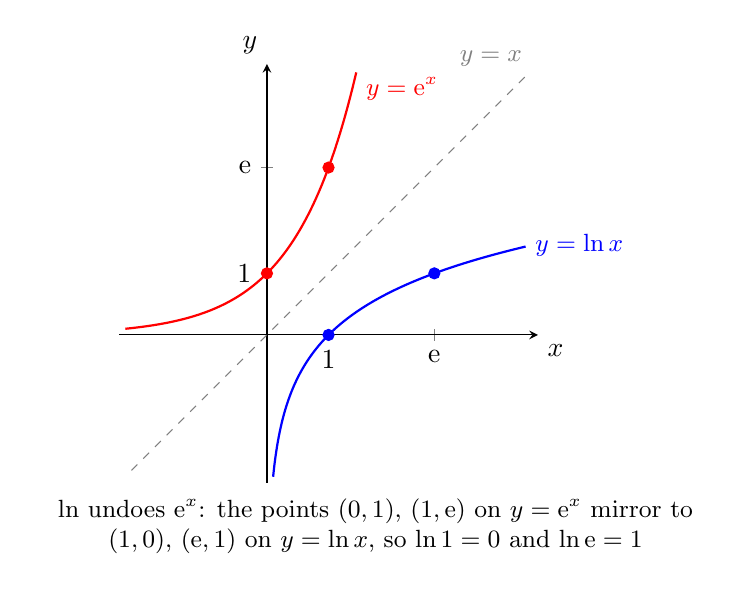
\begin{tikzpicture}
	\begin{axis}[
		axis lines=middle,
		axis equal image,
		xmin=-2.4, xmax=4.4,
		ymin=-2.4, ymax=4.4,
		xtick={1,2.718}, xticklabels={$1$,$\mathrm{e}$}, ytick={1,2.718}, yticklabels={$1$,$\mathrm{e}$},
		xlabel={$x$}, ylabel={$y$},
		xlabel style={below right}, ylabel style={above left},
		samples=200, smooth, clip=false,
		width=8cm
		]
		\addplot[gray, dashed, domain=-2.2:4.2] {x};
		\addplot[thick, red, domain=-2.3:1.45] {exp(x)};
		\addplot[thick, blue, domain=0.1:4.2] {ln(x)};
		\addplot[only marks, mark=*, red] coordinates {(0,1) (1,2.718)};
		\addplot[only marks, mark=*, blue] coordinates {(1,0) (2.718,1)};
		\node[red, anchor=west, font=\small] at (axis cs:1.45,4.0) {$y=\mathrm{e}^x$};
		\node[blue, anchor=west, font=\small] at (axis cs:4.2,1.45) {$y=\ln x$};
		\node[gray, anchor=south east, font=\small] at (axis cs:4.3,4.2) {$y=x$};
	\end{axis}
	\node[anchor=north, font=\small, align=flush center, text width=8.6cm] at ([yshift=-2pt]current axis.outer south) {$\ln$ undoes $\mathrm{e}^x$: the points $(0,1)$, $(1,\mathrm{e})$ on $y=\mathrm{e}^x$ mirror to $(1,0)$, $(\mathrm{e},1)$ on $y=\ln x$, so $\ln 1=0$ and $\ln \mathrm{e}=1$};
\end{tikzpicture}
\end{document}
